% Options for packages loaded elsewhere
\PassOptionsToPackage{unicode}{hyperref}
\PassOptionsToPackage{hyphens}{url}
\PassOptionsToPackage{dvipsnames,svgnames,x11names}{xcolor}
%
\documentclass[
  super,
  preprint,
  3p]{elsarticle}

\usepackage{amsmath,amssymb}
\usepackage{iftex}
\ifPDFTeX
  \usepackage[T1]{fontenc}
  \usepackage[utf8]{inputenc}
  \usepackage{textcomp} % provide euro and other symbols
\else % if luatex or xetex
  \usepackage{unicode-math}
  \defaultfontfeatures{Scale=MatchLowercase}
  \defaultfontfeatures[\rmfamily]{Ligatures=TeX,Scale=1}
\fi
\usepackage{lmodern}
\ifPDFTeX\else  
    % xetex/luatex font selection
\fi
% Use upquote if available, for straight quotes in verbatim environments
\IfFileExists{upquote.sty}{\usepackage{upquote}}{}
\IfFileExists{microtype.sty}{% use microtype if available
  \usepackage[]{microtype}
  \UseMicrotypeSet[protrusion]{basicmath} % disable protrusion for tt fonts
}{}
\makeatletter
\@ifundefined{KOMAClassName}{% if non-KOMA class
  \IfFileExists{parskip.sty}{%
    \usepackage{parskip}
  }{% else
    \setlength{\parindent}{0pt}
    \setlength{\parskip}{6pt plus 2pt minus 1pt}}
}{% if KOMA class
  \KOMAoptions{parskip=half}}
\makeatother
\usepackage{xcolor}
\setlength{\emergencystretch}{3em} % prevent overfull lines
\setcounter{secnumdepth}{5}
% Make \paragraph and \subparagraph free-standing
\ifx\paragraph\undefined\else
  \let\oldparagraph\paragraph
  \renewcommand{\paragraph}[1]{\oldparagraph{#1}\mbox{}}
\fi
\ifx\subparagraph\undefined\else
  \let\oldsubparagraph\subparagraph
  \renewcommand{\subparagraph}[1]{\oldsubparagraph{#1}\mbox{}}
\fi


\providecommand{\tightlist}{%
  \setlength{\itemsep}{0pt}\setlength{\parskip}{0pt}}\usepackage{longtable,booktabs,array}
\usepackage{calc} % for calculating minipage widths
% Correct order of tables after \paragraph or \subparagraph
\usepackage{etoolbox}
\makeatletter
\patchcmd\longtable{\par}{\if@noskipsec\mbox{}\fi\par}{}{}
\makeatother
% Allow footnotes in longtable head/foot
\IfFileExists{footnotehyper.sty}{\usepackage{footnotehyper}}{\usepackage{footnote}}
\makesavenoteenv{longtable}
\usepackage{graphicx}
\makeatletter
\def\maxwidth{\ifdim\Gin@nat@width>\linewidth\linewidth\else\Gin@nat@width\fi}
\def\maxheight{\ifdim\Gin@nat@height>\textheight\textheight\else\Gin@nat@height\fi}
\makeatother
% Scale images if necessary, so that they will not overflow the page
% margins by default, and it is still possible to overwrite the defaults
% using explicit options in \includegraphics[width, height, ...]{}
\setkeys{Gin}{width=\maxwidth,height=\maxheight,keepaspectratio}
% Set default figure placement to htbp
\makeatletter
\def\fps@figure{htbp}
\makeatother

\makeatletter
\makeatother
\makeatletter
\makeatother
\makeatletter
\@ifpackageloaded{caption}{}{\usepackage{caption}}
\AtBeginDocument{%
\ifdefined\contentsname
  \renewcommand*\contentsname{Table of contents}
\else
  \newcommand\contentsname{Table of contents}
\fi
\ifdefined\listfigurename
  \renewcommand*\listfigurename{List of Figures}
\else
  \newcommand\listfigurename{List of Figures}
\fi
\ifdefined\listtablename
  \renewcommand*\listtablename{List of Tables}
\else
  \newcommand\listtablename{List of Tables}
\fi
\ifdefined\figurename
  \renewcommand*\figurename{Figure}
\else
  \newcommand\figurename{Figure}
\fi
\ifdefined\tablename
  \renewcommand*\tablename{Table}
\else
  \newcommand\tablename{Table}
\fi
}
\@ifpackageloaded{float}{}{\usepackage{float}}
\floatstyle{ruled}
\@ifundefined{c@chapter}{\newfloat{codelisting}{h}{lop}}{\newfloat{codelisting}{h}{lop}[chapter]}
\floatname{codelisting}{Listing}
\newcommand*\listoflistings{\listof{codelisting}{List of Listings}}
\makeatother
\makeatletter
\@ifpackageloaded{caption}{}{\usepackage{caption}}
\@ifpackageloaded{subcaption}{}{\usepackage{subcaption}}
\makeatother
\makeatletter
\@ifpackageloaded{tcolorbox}{}{\usepackage[skins,breakable]{tcolorbox}}
\makeatother
\makeatletter
\@ifundefined{shadecolor}{\definecolor{shadecolor}{rgb}{.97, .97, .97}}
\makeatother
\makeatletter
\makeatother
\makeatletter
\makeatother
\journal{Journal Name}
\ifLuaTeX
  \usepackage{selnolig}  % disable illegal ligatures
\fi
\usepackage[]{natbib}
\bibliographystyle{elsarticle-num}
\IfFileExists{bookmark.sty}{\usepackage{bookmark}}{\usepackage{hyperref}}
\IfFileExists{xurl.sty}{\usepackage{xurl}}{} % add URL line breaks if available
\urlstyle{same} % disable monospaced font for URLs
\hypersetup{
  pdftitle={Ecosistemas Marinos Vulnerables},
  pdfauthor={Victoria Escobar Toro},
  pdfkeywords={Corales, EMV},
  colorlinks=true,
  linkcolor={blue},
  filecolor={Maroon},
  citecolor={Blue},
  urlcolor={Blue},
  pdfcreator={LaTeX via pandoc}}

\setlength{\parindent}{6pt}
\begin{document}

\begin{frontmatter}
\title{Ecosistemas Marinos Vulnerables \\\large{Corales y esponjas} }
\author[1]{Victoria Escobar Toro%
%
}
 \ead{victoria.escobar@ifop.cl} 

\affiliation[1]{organization={Instituto de Fomento
Pesquero, Departamento de Evaluacion de Pesquerias},addressline={Avenida
Blanco Encalada 839},city={Valparaiso},postcodesep={}}

\cortext[cor1]{Corresponding author}

        
\begin{abstract}
An exploration of the databases of presence records was carried out
during the period includeAn exploration of the databases of presence
records was carried out during the period included between 2017 and 2022
of the species present in the catches of Chilean industrial vessels with
scientific observers onboard. The registered species belong to the
vulnerable taxonomic groups and indicators of EMV according to the
classification of Van Ofwegen (2014) and the records obtained in Bernal
et al., 2014, corresponding to corals, sponges, depth stars and actinia.
\end{abstract}





\begin{keyword}
    Corales \sep 
    EMV
\end{keyword}
\end{frontmatter}
    \ifdefined\Shaded\renewenvironment{Shaded}{\begin{tcolorbox}[borderline west={3pt}{0pt}{shadecolor}, breakable, boxrule=0pt, frame hidden, interior hidden, enhanced, sharp corners]}{\end{tcolorbox}}\fi

Las observaciones provienen de 19 embarcaciones que operaron entre los
a�os 2017 - 2022, pertenecientes a las flotas industriales de la
Pesqueria demersal centro sur, Pesqueria sur austral, Pesqueria de
espinel de bacalao de profundidad y la Pesqueria de crustaceos
demersales (industrial y artesanal). La cobertura de estos viajes fue
del 24,3\%, durante estos viajes se realizaron 28.637 lances, de los
cuales en el 0,03\% se registro la presencia de actinias, esponjas,
corales petreos, corales blandos y estrellas de profundidad.

Se realizo una exploracion de las bases de datos de registros de
presencia durante el periodo comprendido entre el 2017 y 2022 de las
especies presentes en las capturas de embarcaciones industriales con
observadores cientificos. Las especies registradas pertenecen a los
grupos taxonomicos vulnerables e indicadores de EMV de acuerdo a la
clasificacion de Van Ofwegen (2014) y los registros obtenidos en Bernal
et al.~2014, correspondientes a corales, esponjas, estrellas de
profundidad y actinias (Figura 1)

De la serie presentada, entre las especies indicadoras de habitat de
ecosistemas marinos vulnerables (EMV) y especies vulnerables, las
especies mas recurrentes en los registros de los observadores
(presencia), para las pesquerias fueron los corales petreos (30,5\%),
secundariamente las estrellas de profundidad (Hippasteria phrygiana),
esponjas (Spongia sp) con un 19\% respectivamente y las actinias con un
17\% (Figura 2).

Espacialmente, estas especies se distribuyeron entre las latitudes
29�42�30'' LS -- 57�15�00'' LS. De la clase Anthozoa, los corales
petreos correspondieron al taxon mas recurrente en las pesquerias de
arrastre fabrica y de espinel de bacalao con una amplia representaci�n
espacial (Figuras 3).

\begin{figure}

{\centering 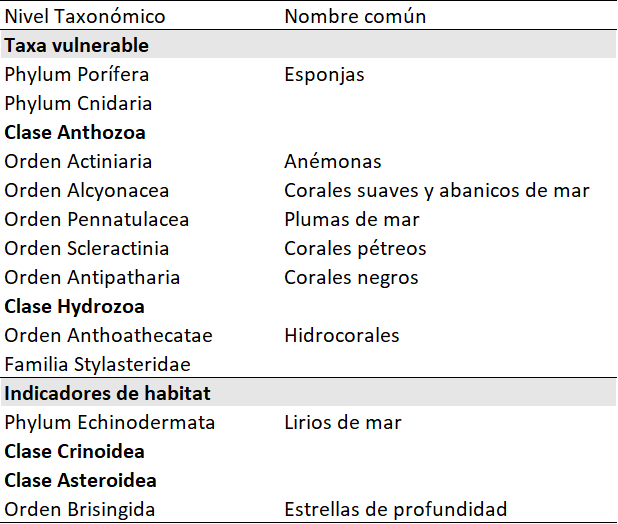
\includegraphics[width=3.85417in,height=\textheight]{especies.png}

}

\caption{Grupos taxonomicos evaluados como vulnerables}

\end{figure}

\begin{figure}

{\centering 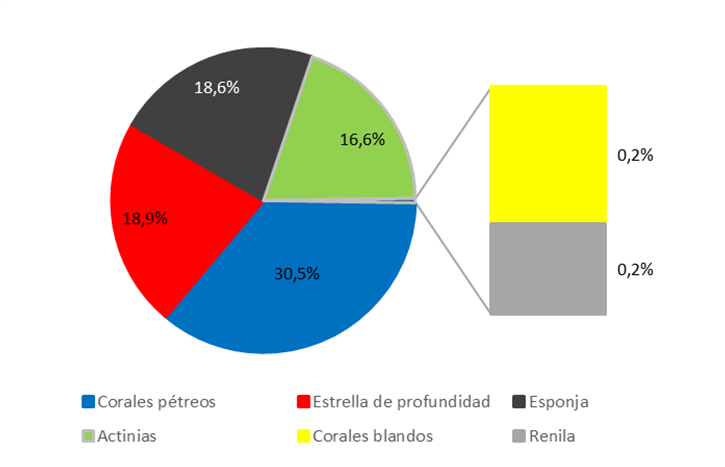
\includegraphics{grafico-pie.png}

}

\caption{Porcentaje de registros de especies indicadoras de EMV y
taxones vulnerables en las pesquerias chilenas}

\end{figure}

\begin{figure}

{\centering 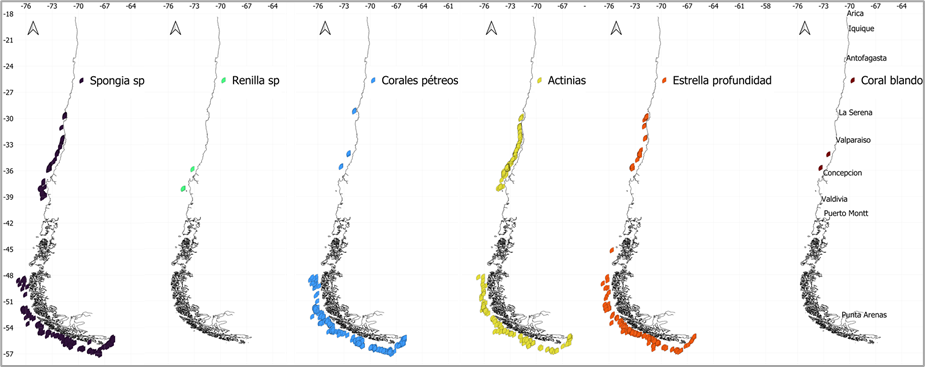
\includegraphics{mapa.png}

}

\caption{Presencia espacial de invertebrados marinos observados y
capturados en las operaciones de pesca, periodo 2017-2022}

\end{figure}


  \bibliography{bibliography.bib}


\end{document}
